\section{Accouting for multiscale data with multiattribute models}

\begin{frame}
  \frametitle{Why Multi-attribute Networks?}
  \framesubtitle{Joint work with E. Kolaczyk (Boston) and C.  Ambroise
    (Évry)}

  \begin{tikzpicture}
    \tikzstyle{every state}=[fill=orange!70!white,draw=none,text=white]
      
    \node[state] (dna) at (0,0) {DNA};
    \node[state] (rna) at (4,0) {RNA};
    \node[state] (proteins) at (8,0) {Proteins};
    \node[state] (tf) at (6,-1.2) {TF};
    \node[state] (enzyme) at (9,-2) {Enz.};
    \node[draw=none,text=white,fill=genecolor, scale=0.75] (gene) at (0.5,0.5) {genes};
    
    \path
    (dna) edge [->] node[above] {transcription} (rna) 
    (rna) edge [->] node[above] {translation} (proteins) 
    (dna) edge [loop left,->] node[below=10pt] {replication} (dna) 
    (proteins) edge [->] node {} (tf) 
    (proteins) edge [->] node {} (enzyme) 
    (proteins) edge [loop right, ->] node[above left=10pt] {\textcolor{red}{may bind}} (proteins) 
    (tf) edge [bend left, ->] node[midway] {\textcolor{genecolor}{regulates}} ($(rna.west) -(5mm,0)$)
    (rna) edge [-,line width=2pt,draw=white,bend left] ($(rna.west) -(15mm,0)$)
    (rna) edge [bend left, ->] node {\textcolor{genecolor}{regulates}} ($(rna.west) -(15mm,0)$);
  \end{tikzpicture}    

  \vspace{-.5cm}

  \begin{block}{Data integration}
    \begin{itemize}
    \item  Omic technologies  can  profile  cells at  \alert{different
        levels}: DNA, RNA, protein, chromosomal, and functional.
    \item \alert{multiple} molecular  profiles \alert{combined} on the
      same set of biological samples can be \textit{synergistic}.
    \end{itemize}
  \end{block}
  
\end{frame}

\begin{frame}
  \frametitle{Multiattribute GGM}

    Consider e.g. some $p$ genes of interest and the $K=2$ omic experiments
    \begin{enumerate}
    \item $X_{i1}$ is the expression profile of gene $i$ (transcriptomic data),
    \item $X_{i2}$ is the corresponding protein concentration (proteomic data).
    \end{enumerate}

    \vfill

  \begin{block}{Define a block-wise precision matrix}
      \vspace{-.25cm}
      \begin{itemize}
      \item  $X =  (X_1,  \dots,  X_p)^T \sim  \mathcal{N}(\mathbf{0},
        \bSigma)$ in $\Rset^{pK}$,
      \item $X_i=(X_{i1},\dots,X_{iK})^\intercal \in \mathbb{R}^K$.
      \end{itemize}
      \[
      \invcov = \bSigma^{-1} = \begin{bmatrix}
        \invcov_{11} & & \invcov_{1p} \\
        & \ddots & \\
        \invcov_{p1} & & \invcov_{pp} \\
      \end{bmatrix}, \qquad  \invcov_{ij} \in \mathcal{M}_{K,K},
      \ \forall (i,j)\in\mathcal{P}^2.
      \]
    \end{block}

    \vfill

    \begin{beamerboxesrounded}[upper=sur:head,lower=sur:bloc,shadow=true]{Graphical Interpretation}
      Define  $\mathcal{G}=(\mathcal{P},\mathcal{E})$   as  \alert{the
        multivariate analogue} of the {\it conditional graph}:
      \vspace{-.25cm}
      \begin{equation*}
        (i,j)\in    \mathcal{E}    \Leftrightarrow    \invcov_{ij}    \ne
        \mathbf{0}_{KK}.
      \end{equation*}
    \end{beamerboxesrounded}

\end{frame}

\begin{frame}
  \frametitle{Multiattribute GGM as multivariate regression}

  \begin{block}{Multivariate analysis view point}
    Straightforward algebra and we have
    \begin{equation*}
      \label{eq:condK}
      X_j \, |\,  X_{\backslash j}  = x \sim  \mathcal{N}(- \invcov_{jj}^{-1}\invcov_{j
        \backslash j} x , \invcov_{ii}^{-1})\enskip.
    \end{equation*}
    or   equivalently,    letting   $\displaystyle    \mathbf{B}_j^T   =
    -\invcov_{jj}^{-1} \invcov_{i\backslash j}$,
    \begin{equation*}
      \label{eq:condK}
      X_j \, |\, X_{\backslash j} = \mathbf{B}_j^T X_{\backslash j} +
      \boldsymbol\varepsilon_j \quad \boldsymbol\varepsilon_j
      \sim \mathcal{N}(\mathbf{0},\invcov_{ii}^{-1}), \quad \boldsymbol\varepsilon_j \perp X.
    \end{equation*}
  \end{block}

    \begin{colormixin}{60!white}
      \begin{block}{Remembering the univariate case?}
        \[
        X_j   |    X_{   \setminus    j}   =   -    \sum_{\alert{k   \in
            \text{neighbors}(j)}} \frac{\invcov_{jk}}{\invcov_{jj}}  X_j +
        \varepsilon_j,\quad              \varepsilon_j              \sim
        \mathcal{N}(0,\invcov_{jj}^{-1}), \quad \varepsilon_j \perp X.
        \]
      \end{block}
    \end{colormixin}
\end{frame}

\begin{frame}
  \frametitle{Multivariate neighborhood selection} 

  \begin{block}{The penalized multivariate regression approach}
    For each node /gene, recover its neighborhood by solving 
    \begin{equation*}
      \arg  \min_{\mathbf{B}_j  \in  \mathcal{M}_{(p-1)K,K}}  \frac{1}{2n} \left\|
        \bX_j - \bX_{\backslash j}\bB_j\right\|_F^2 +
      \lambda \ \text{Pen}(\bB_j),
    \end{equation*}
  \end{block}
  
  \vfill
  
  \begin{block}{Choice of penalty}
    Group-based   penalty   to   activate  the   set   of   attributes
    simultaneously on a given link:
    \begin{equation*}
      \text{Pen}(\bB_j) =       \sum_{k \neq j}  \|\bB_j^{(k)}\|  \enskip  ,
      \quad \bB_j^{(k)} \in \mathcal{M}_{KK}
    \end{equation*}
    \begin{itemize}
    \item  \alert{$\|M\|=   \|M\|_F=\left(  \sum_{i,j}  M_{ij}^2\right)^{1/2}$,
        the Frobenius norm},
    \item  $\|M\|=  \|M\|_\infty=  \max_{i,j}{|M_{ij}|}$, the  sup  norm
      (shared magnitude),
    \item $\|M\|= \|M\|_\star=\sum \mathrm{eig}(M)$, the nuclear norm
      (rank penalty).
    \end{itemize}      
  \end{block}
\end{frame}

\begin{frame}
  \frametitle{Breast cancer data: application}

  Two cohorts with both proteomic and transcriptomic data
  \begin{enumerate}
    \item \emphase{NCI-60}: $n=60$ diverse human cancer cell lines, $p=91$
    \item  \emphase{RATHER}: $n=100$ sample from patients with breast cancer, $p=117$
  \end{enumerate}

\begin{figure}[htbp!]
  \centering
  \begin{tabular}{@{}cc@{}}
   RATHER & NCI-60 \\
    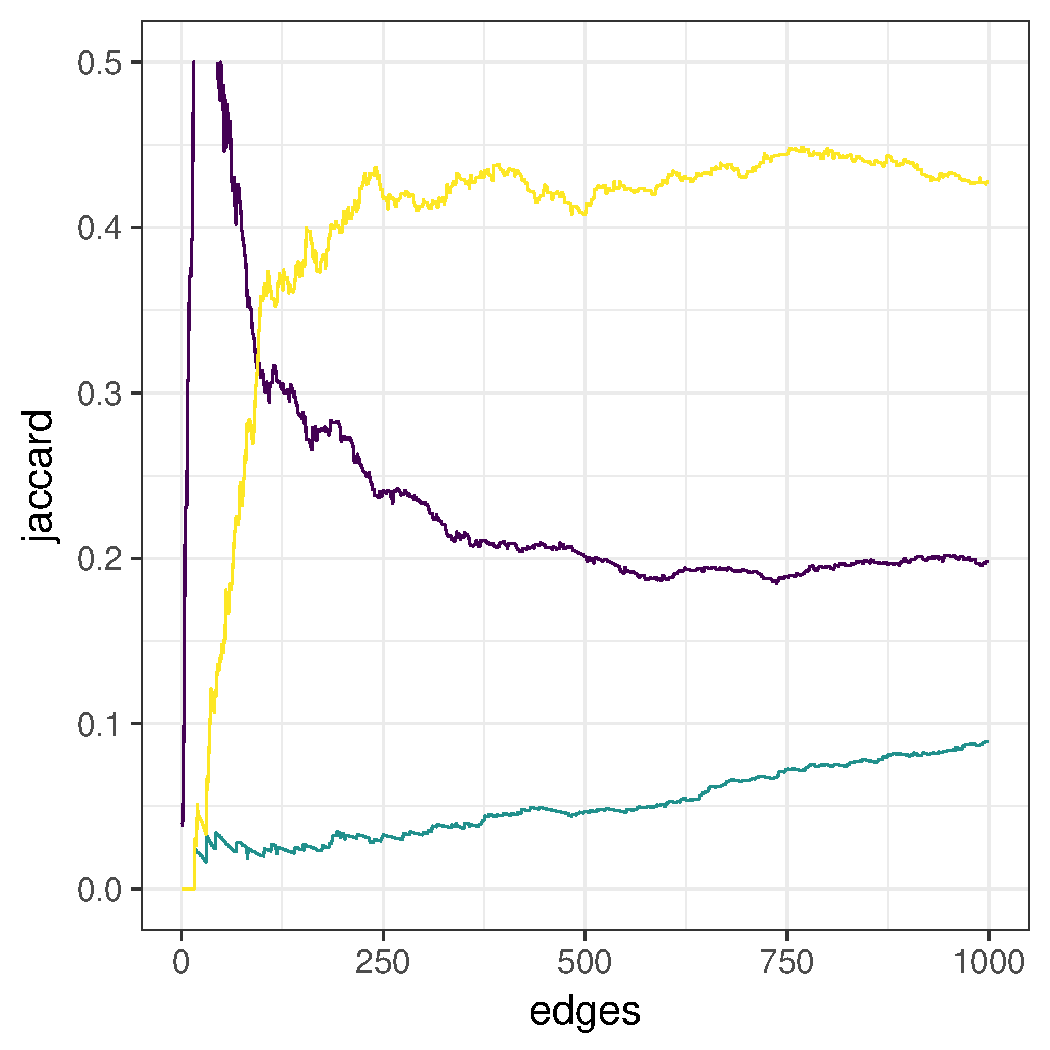
\includegraphics[width=.35\textwidth]{figures/jaccard_RATHER}
  & 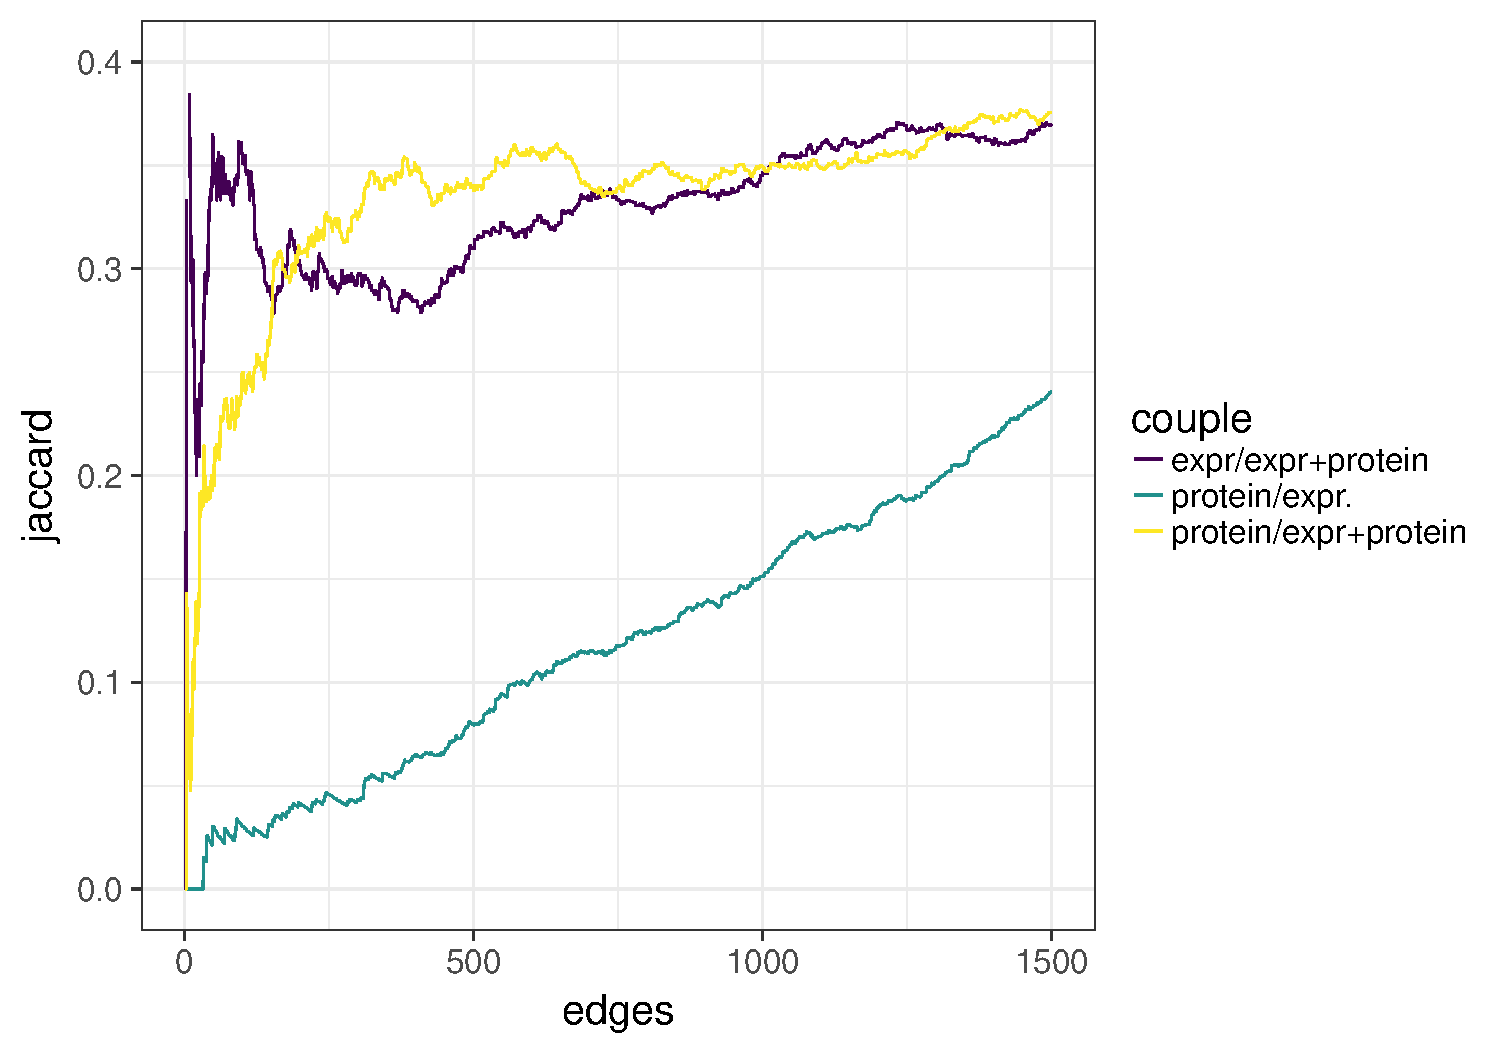
\includegraphics[width=.5\textwidth]{figures/jaccard_NCI60}
  \end{tabular}
  \caption{Jaccard's similarity index
    $J(A,B) = \frac{\left|A\cap B\right|}{\left|A\cup B\right|}$
    between uni-attribute and multiattribute networks, for RATHER and
    NCI60 data set: multiattribute networks share a high Jaccard
    index with both uni-attribute networks.}
  \label{fig:jaccard}
\end{figure}

\end{frame}

\begin{frame}
  \frametitle{Inferred networks}
  
\begin{figure}[htbp!]
  \centering
  \begin{tabular}{@{}lccc@{}}
    & proteomic network  & transcriptomic network  & multiattribute network \\
    \rotatebox{90}{\hspace{1.2cm}NCI60} 
    & 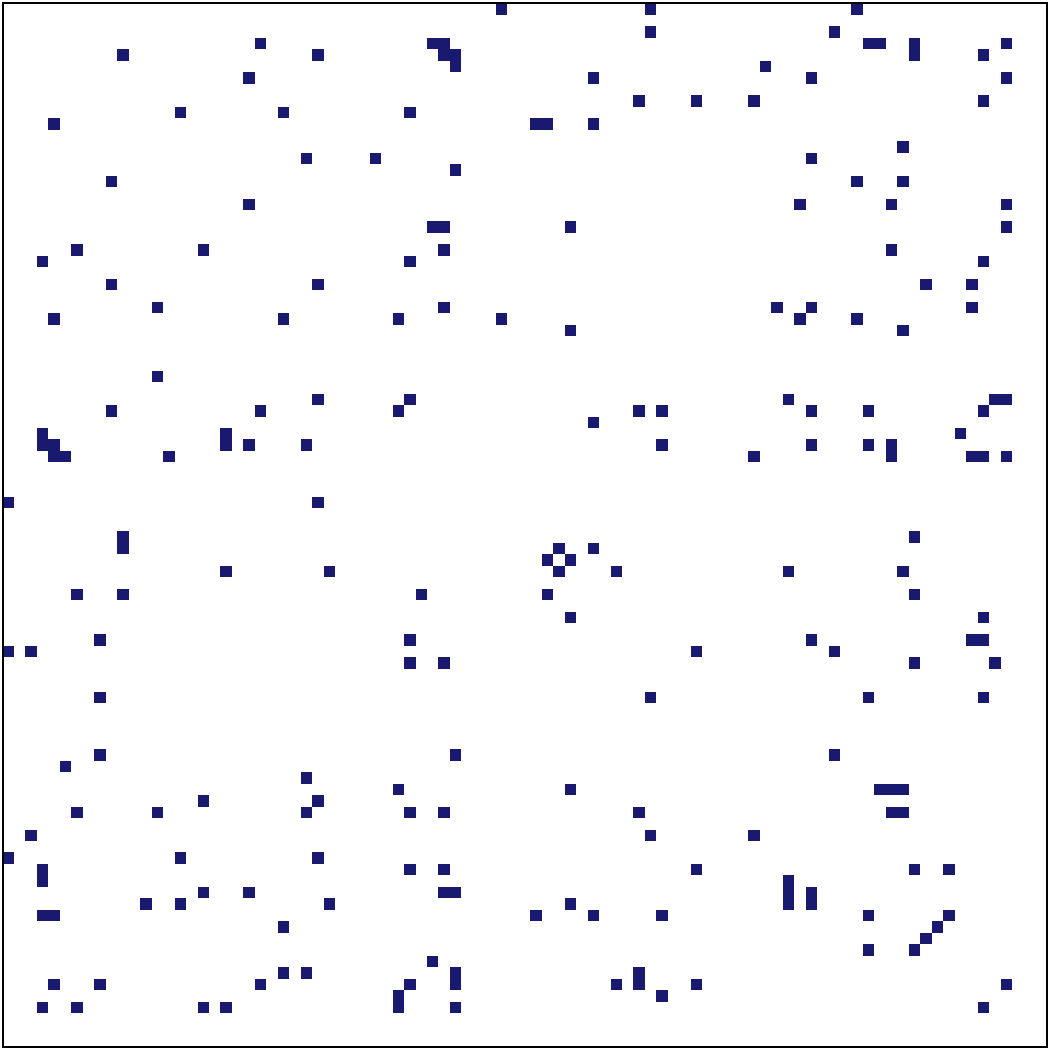
\includegraphics[width=.25\textwidth]{figures/protNet_NCI60}
    & 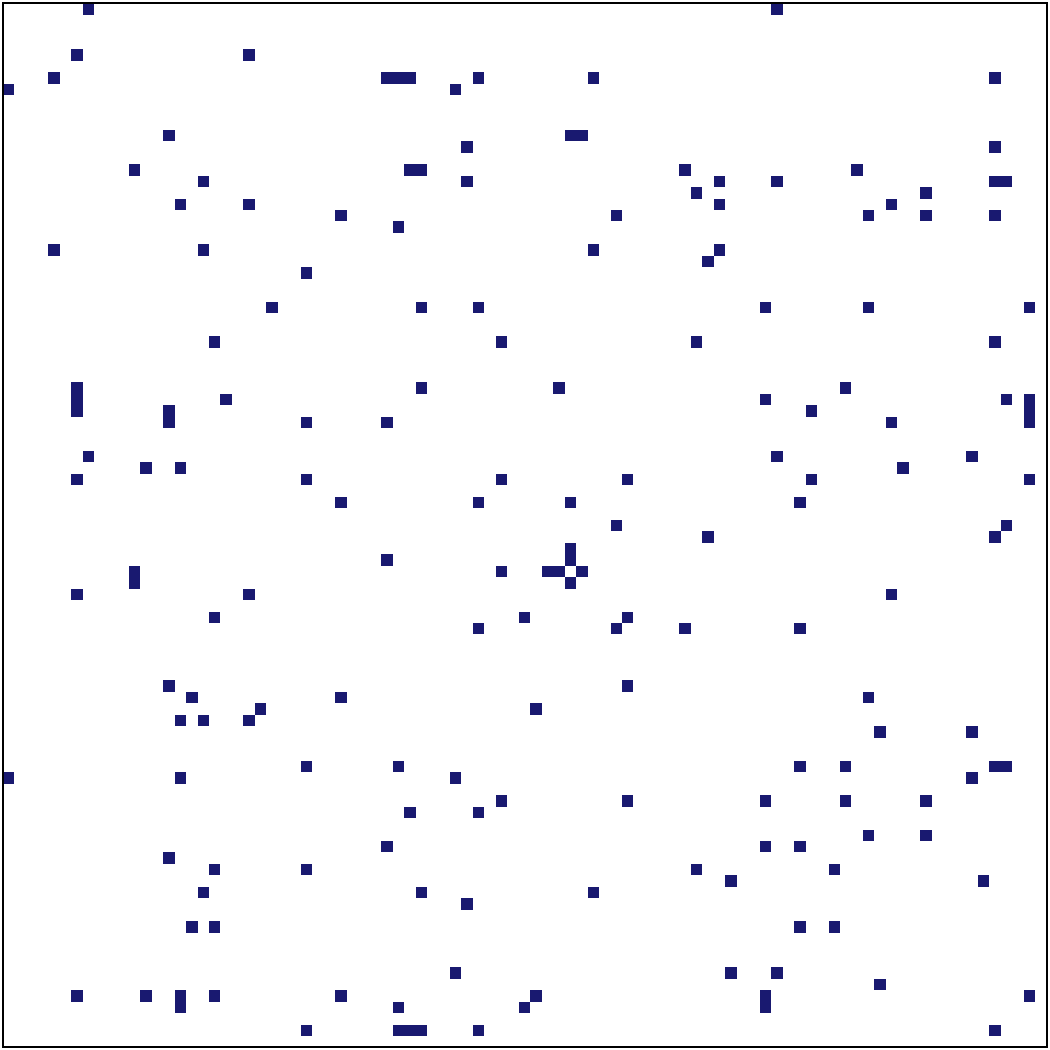
\includegraphics[width=.25\textwidth]{figures/exprNet_NCI60}
    & 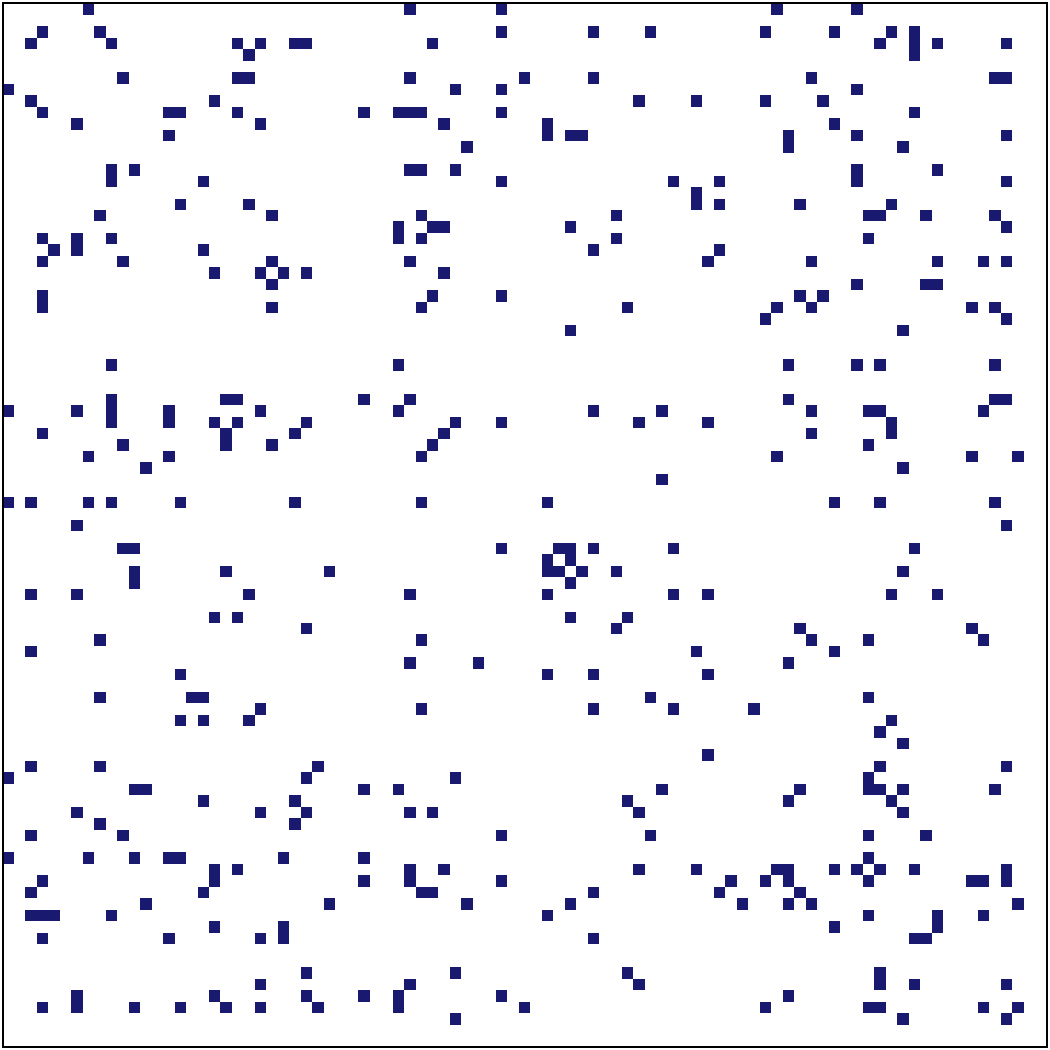
\includegraphics[width=.25\textwidth]{figures/bivarNet_NCI60} \\
    \rotatebox{90}{\hspace{1.2cm}RATHER} 
    & 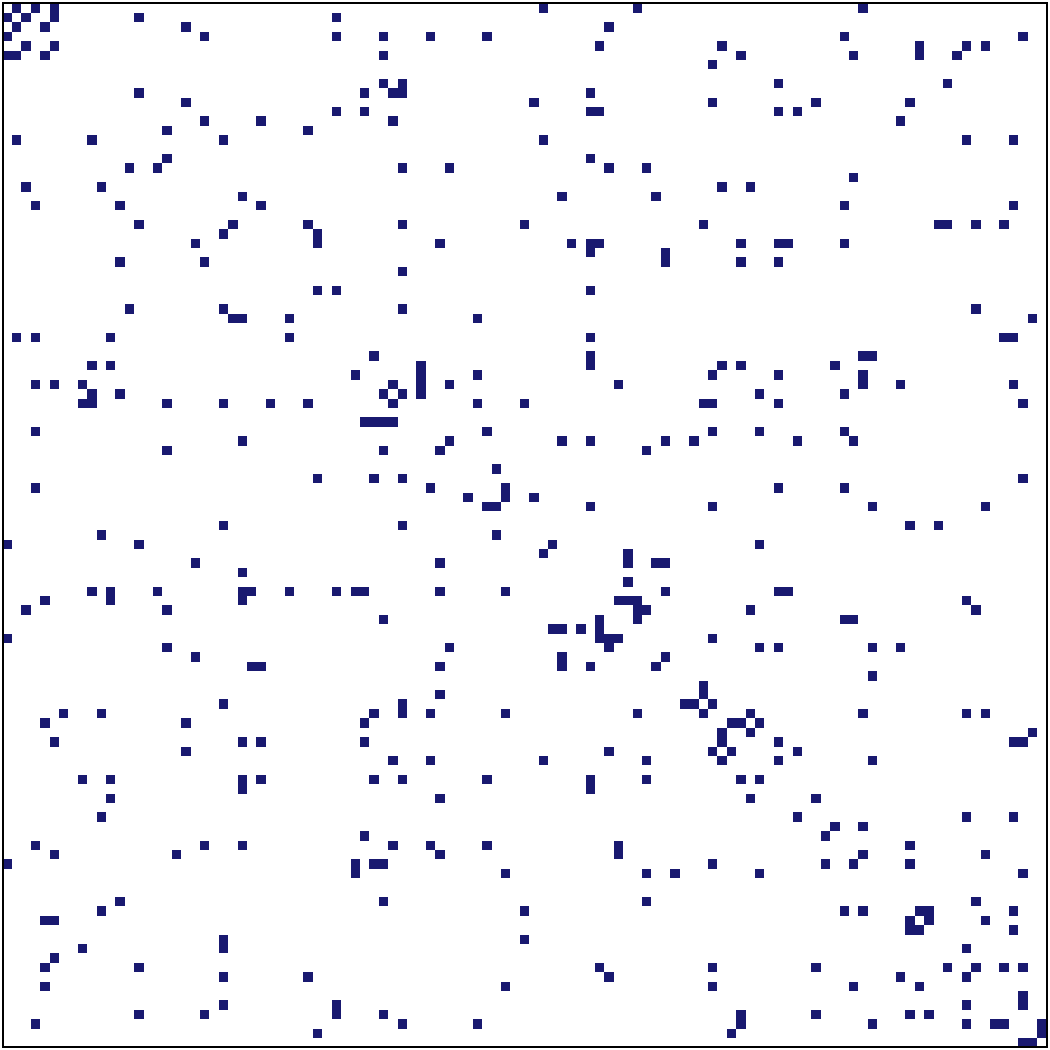
\includegraphics[width=.25\textwidth]{figures/protNet_RATHER}
    & 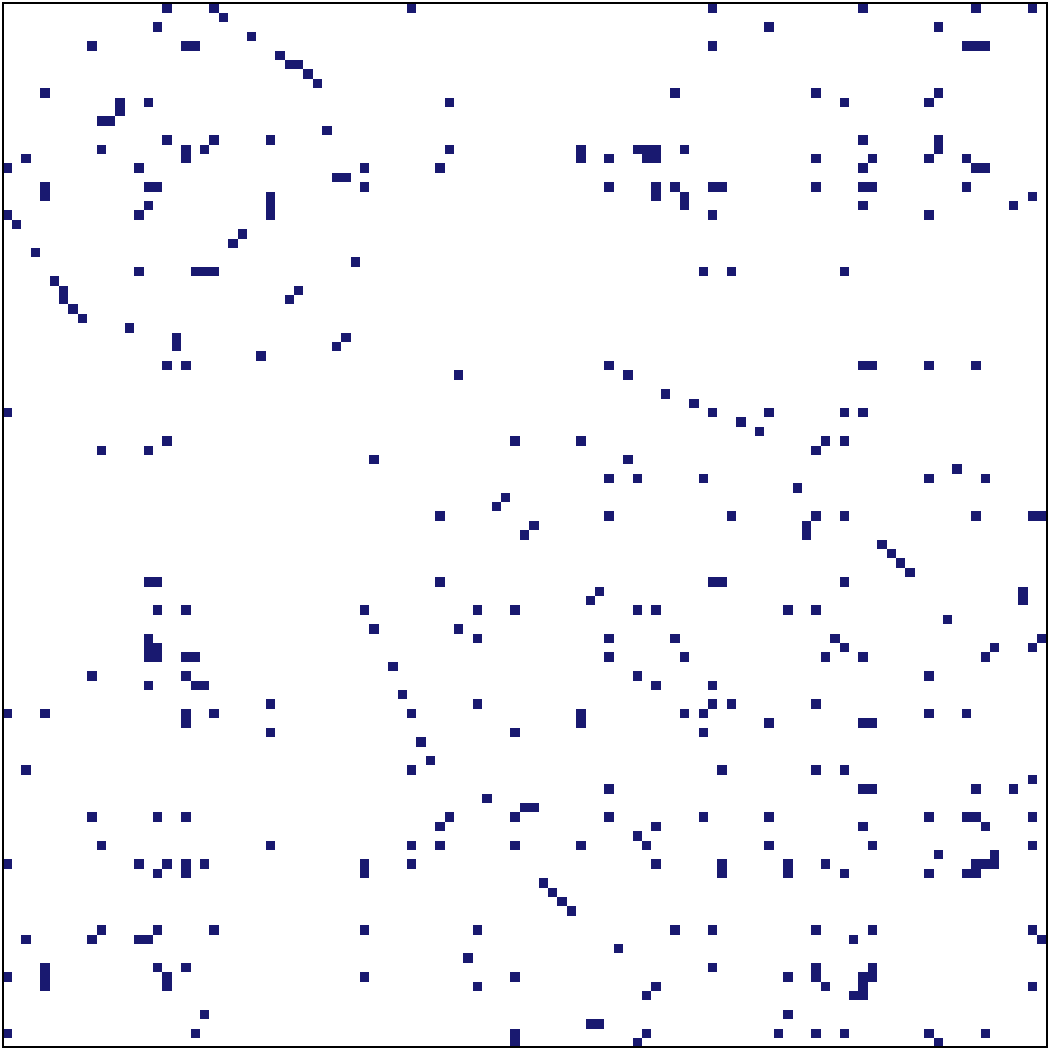
\includegraphics[width=.25\textwidth]{figures/exprNet_RATHER}
    & 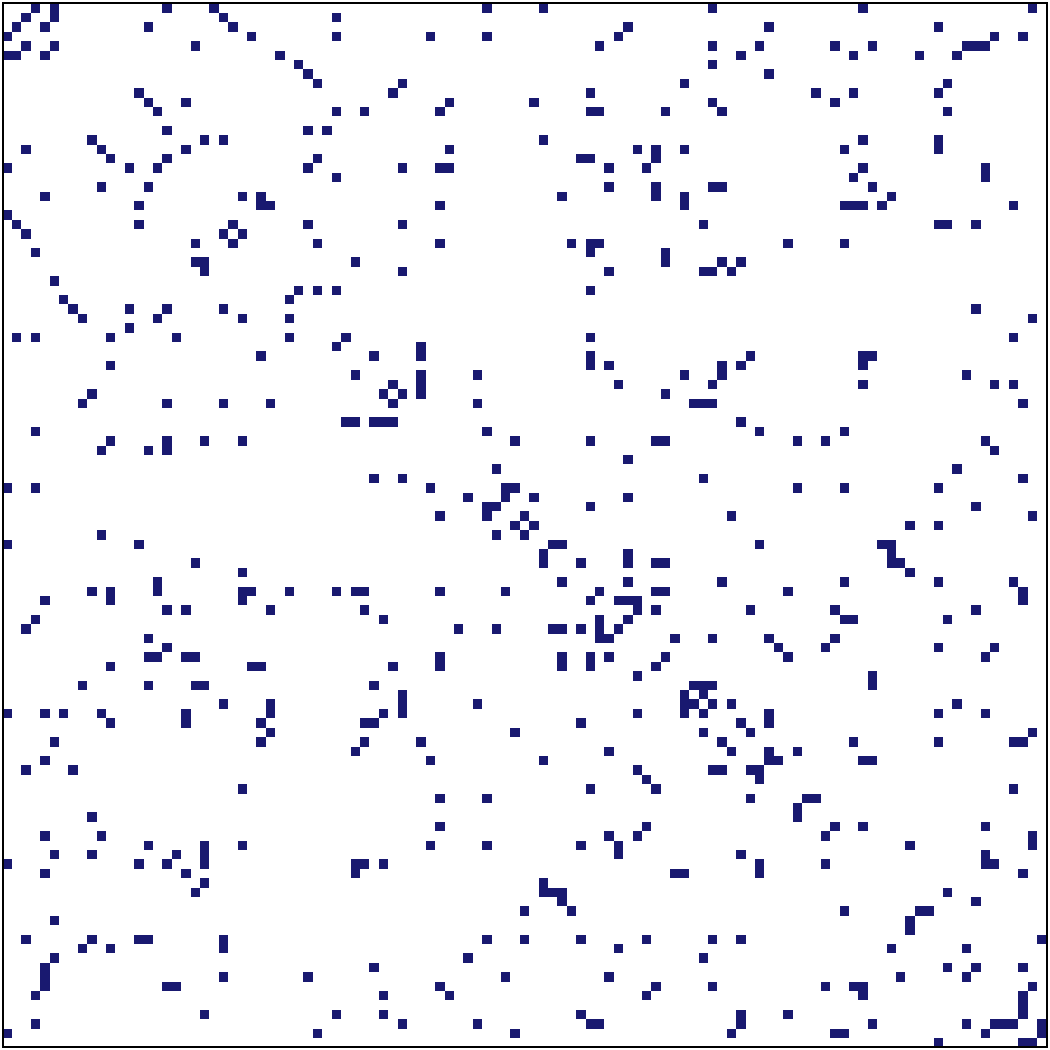
\includegraphics[width=.25\textwidth]{figures/bivarNet_RATHER} \\
  \end{tabular}
  \caption{Uni-attribute and multiattribute networks inferred on both
    NCI60 and RATHER dataset. The number of neighbors of each entity
    is chosen by cross-validation. Multiattribute networks catch motif
    found in the uniattribute counterparts.}
  \label{fig:networks}
\end{figure}

\end{frame}

